% !TEX root = MAIN.tex




\section{Data-driven Mutation Testing: DAMTE} % (fold)
\label{sec:data:test_suite_augmentation}



The \INDEX{test suite augmentation process} it consists of four activities \INDEX{Identify Test Inputs}, \INDEX{Generate Test Oracles}, \INDEX{Execute the SUT}, \INDEX{Fix the SUT}. It has the objective of increasing the score generated by the mutation analysis process.

FAQAS focussed on a methodology (i.e., data-driven mutation testing, \INDEX{DAMTE}) that specifies how to rely on KLEE to generate test inputs that increase the fault model coverage and the mutation operation coverage.
FAQAS does not address increasing the mutation score because infeasible in automated manner.
We recall that two might be the reasons for a low MS: poor oracle quality and missing test input sequences.
If the low mutation score is due to poor oracle quality, manual work is needed because automated approaches to automatically generate test oracles in the presence of system or integration test suites are not available. 
If the low mutation score is due to missing test input sequences (i.e., the software does not reach the state in which it could kill the mutant), manual work is required because existing test generation approaches (e.g., KLEE) might suffer from scalability problem that prevent bringing the system into a desired state; also, they cannot deal with systems whose components communicate through channels. 

For the cases targeted by FAQAS (i.e.,
in the presence of fault model coverage and mutation operation coverage below 100\%), test generation has the objective of generating test inputs that enable the application of all the mutation operators. 
We thus rely on an  \INDEX{extended data mutation probe} that
invokes a version of the data mutation API that instead of mutating the data targeted by the mutation operator not covered by the fault model, includes a reachability assertion that is used to make KLEE find a test input that reaches the mutant code. The test input shall then be inspected by the engineer, who will need then to integrate it into his test suite.
%Figure~\ref{fig:dataDrivenTestSuiteAugmentationB} exemplifies how data driven mutation testing works, for the producer consumer and client-server cases.
%
%
%
%
%\begin{figure}[h]
%  \centering
%    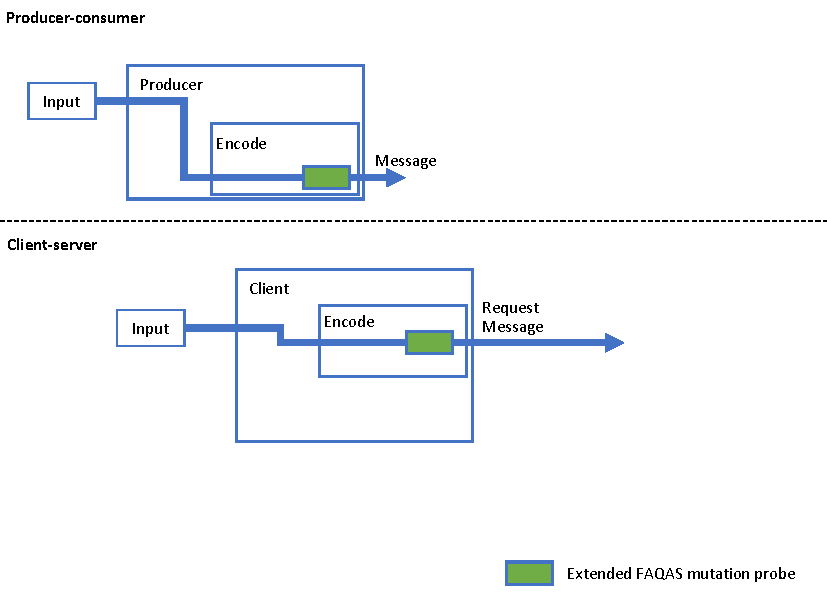
\includegraphics[width=14cm]{images/dataDrivenTestSuiteAugmentationB}
%      \caption{Data-driven mutation analysis for different architectures.}
%      \label{fig:dataDrivenTestSuiteAugmentationB}
%\end{figure}







